\chapter{State of the art}
\label{chap:stateoftheart}

\section{Deployment tool for an UAV network}
\label{sec:stateoftheart:deploymenttool}

Calculating electromagnetic exposure requires knowledge about the area. The position of base stations need to be known,
 the transmission power used by the antenna and how far the user is separated from this base stations are only a few parameters
 that have to be considered.

The WAVES research group at UGent has developed a deployment tool for disaster scenarios with the aid of UAVs \cite{J2}.
The idea of this UAV-aided emergency network is that in case of a disaster, the existing network might be damaged and won't be able 
to handle all users who are trying to reconnect to the backbone network. 
The tool makes a fast deployable network possible by attaching femtocells to UAVs, so-called \gls{UABS}s.
The tool will orchestrate the \gls{UABS}s over the disaster area. This tool is thus a suitable starting point and works as follows:

%The optimal placement for each \gls{UABS} needs to be defined to make sure that as many users as possible are properly reconnected to the backbone network while satisfying certain restrictions. 
%To make these calculations as realistic as possible the architecture of the several buildings present in the area is described in a shapefile. 
%A deployment tool calculates the optimal position of the \gls{UABS} by taking the 3D models of the building into account along with some femtocell specifications and user distribution. This deployment tool is developed by the WAVES research group, a department within Ghent University.

The deployment tool will try to calculate the optimal placement for each \gls{UABS} and requires therefore a description of the area where the UAV-aided network needs to 
be deployed. This is done with the use of so-called shape files. These files contain three dimensional descriptions of the buildings present in the area and are
key values in approaching results as realistic as possible. Furthermore, the tool also requires a time period and a configuration file containing technical specifications of the type of \gls{UABS} that is being used. 
The tool will thereafter randomly distribute users over the area and assigns a certain bitrate to them. \\
\\
In a second phase, the optimal position for each \gls{UABS} is calculated. This is done by trying to locate a \gls{UABS} above each active user. Two options are possible.
If a fixed flying height is defined, a base stations is placed above each user at the given height, unless a building is obstructing it's location. Then, no base station will be located above that user.
Alternatively to the fixed flying height, a flying margin can be defined which represents the distance between the outdoor user and  the drone.
If the user is inside, this margin will be measured between the drone and the rooftop of that building.
The latter is only allowed if the suggested height remains below the given maximum allowed height. \\
\\
Finally, all \gls{UABS} are sorted on wether they were active or not, followed by the increasing pathloss from each \gls{UABS} to that user.
So the algorithm starts by checking for each active \gls{UABS} if it can cover the user. If this is the case, the user will be connected to this \gls{UABS}. If not,
the second active base station with a (slightly) worse pathloss is considered. If no active base station is suitable, inactive \gls{UABS} are considered. The user remains uncovered if no \gls{UABS}
is found. The reason behind first only considering base stations that are already active, is the hight cost that comes along with each drone. \\
\\
Up till now, the tool has only calculated some suggestions. The effective provisioning is done in the fourth phase where drones are sorted by the amount of users they cover. As long as \gls{UABS}
are available in the facility where they reside, \gls{UABS} are provisioned and its users are marked as covered.


\section{Electromagnetic exposure}

\subsection{Electromagnetic field radiation} % (fold)
\label{sub:emf}
People in a telecommunication network are exposed to far field electromagnetic radiation originating from base stations and other \gls{UE}. 
Network planners need to make sure that the electromagnetic fields (expressed in V/m) do not exceed limitations enforced 
by the government. These limits are location dependent. The European Union recommend the guidelines as defined by the \gls{ICNIRP} which limits electromagnetic exposure to 61 V/m.
Each european country needs to decide for themselves which limitations to enforce. Belgium for example delegated this responsibility to Flanders, Brussels and Wallonia \cite{J23}.

The used deployment tool is applied in Ghent, a Flemish city in Belgium. The standards defined by the Flemish government are therefore applicable.
They state that in the 2.6 Ghz frequency band, an individual antenna can't exceed 4.5 V/m and the cumulative sum of all fixed sources 31 V/m \cite{S13_normenBelgie}.

\subsection{Specific Absorption Rate}

\gls{SAR} represents the rate that electromagnetic energy is absorbed by human tissue with the thermal effect as it's most important health consequence.
The volume of this tissue is typically 1g or 10g. The Federal Communications Commission of the United States defines regulations based on 1g tissue (indicated as $SAR_{1g}$) 
while the European Union handles the 
10g model ($SAR_{10g}$). $SAR$ values can further be categorized based on the area it covers. 
A first one is whole body \gls{SAR} ($SAR^{wb}$) which is the average absorbed radiation over the entire 
body. The second type is more precisely. Localized \gls{SAR}-values cover only  a part of the human body like the head.
The \gls{ICNIRP} has concluded that the threshold effect for $SAR^{wb}_{10g}$ is at 4 W/kg meaning that any higher absorption rate would overwhelm the \gls{thermoregulatory capacity} of the human body.
Whole body values between 1 and 4 W/kg increase the temperature of human body less than 1°C, which is proven not to be harmful for a healthy human being\cite{J24}.
Thereafter, a safety margin is introduced to tackle unknown variables like experimental errors, increased sensitivity for certain population groups and so on. 
This results in a whole body $SAR_{10g}$ of $0.8 W/kg$ and $2 W/kg$ for localized $SAR_{10g}$ at head and torso area \cite{J23}.

%todo: de 10g slaat al op localized, vandaar dat het maar 10g is, anders is het whole-body
%todo: we kunnen niet sar10gmax gebruiken want This means that the SAR calculations will be worst-case and possibly an overestimation of the real localised SAR. (herwoorden voor plagiaat)
%Human exposure caused by downlink traffic is a not negligible asset. However, telecommunications is not a one-way street. When connecting to a UMTS network, also uplink data caused by the \gls{UE} should be considered.
%\gls{UE} generates, just like femtocells, electromagnetic waves to which a user is exposed. A part of this radiation goes to the femtocell, another part enters the body of its user. How much electormagnic strenghts enters the body is defined as \gls{SAR} and is measured with 10g biological tissue which represents the human skin. This value will from now on be expressed as $SAR_{10g}$. 
%A mobile device induces two types of exposure: local and whole-body. 

\subsection{Related work} % (fold)
\label{sub:general}
The goals of this master dissertation is the investigation of electromagnetic exposure considering all sources. Three types of sources are considered: electromagnetic radiation 
caused by basestations, near field radiation from the user's own device and far field radiation originating from other users their equipment. This electromagnetic radiation is thereafter
absorbed by the human body which will be expressed in \gls{SAR} values.

Several papers exist calculating exposure originating from certain sources, but very limited research has been done covering the whole picture.
In \cite{J6_originalExposureFormula} is described how electromagnetic radiation of several WiFi access points is being calculated. The authors of \cite{J1} used this knowledge 
to investigate electromagnetic exposure originating from basestations in a more outdoor environment. \cite{J10_RDP, J10.1} addresses the fact that 
also \gls{UL} traffic from the user's device should be considered. They therefore investigated indoor exposure. They did not only consider the electromagnetic radiation
but also how much is absorbed by the body which will be expressed as specific absorption rate. Since the authors only covered voice calls,
uplink SAR was expressed in localized SAR values while the downlink traffic is expressed in whole body SAR. With the advent of 5G, paper \cite{J17_kuehn2019modelling} has been 
published, describing how localized SAR values are achieved from all sources. More precisely: all mobile phones and all basestations in the network after which they converted the electromagnetic 
exposure to localized SAR values.
Finally, \cite{J22_plets2015joint} describes how both \gls{UL} and \gls{DL} traffic can be converted in whole body SAR values making it possible to achieve an overall picture. They applied this formula 
however only for the user's own device.

In a realistic network like the used deployment tool, some users are calling while another part is using other types of telecommunication services like browsing the web.
Therefore, all absorbed electromagnetic exposure should be expressed in whole body SAR while still covering all sources.

\section{Optimizing towards electromagnetic exposure and power consumption}
\gls{UABS}s are drones with femtocell base stations attached to it. Drones can remain in the air for only a limited time, which is certainly 
the case when also an antenna needs to be connected to the battery of his carrier. It is therefore
interesting to not only consider electromagnetic exposure of the user but also the power consumption that comes with it. 
However an increasing transmission power of an antenna comes with an increasing electromagnetic exposure. This is not the case considering
both values for an entire network. In fact, the autors from \cite{J1}  prove that both become inversely equivalent.

If a network is optimized towards power consumption, less drones will be provisioned radiating at higher power levels. This is because not only 
the transmission power is considered but also the power needed to keep the drone in the air. Therefore, it is cheaper to cover a user by 
increasing the antennae transmission power of an already activated drone nearby as it therefore prevents the power cost of a new drone.
By increasing the transmission power, also the electomagnetic exposure will increase for users closer to that drone. An exposure optimized
network will therefore faster decide to power up a new drone.

\section{Technologies}
\subsection{Type of drone}

Section \ref{sec:stateoftheart:deploymenttool} described how femtocell antennae will be connected to helicopter drones. Two types of 
drones are considered in \cite{J2}: an off-the-shelf drone affordable by the general public and a more expensive drone. The results in \cite{J2}
show that the second type will require less drones to cover the same number of users and will last longer in the air. The research in this paper
will therefore be done with the usage of the second type. A technical overview of this drone is given in table \ref{table:dronespecs}.

\begin{table}[h!]
\centering
\begin{tabular}{|l|c|l|}
\hline
 Parameter          & value         \\    \hline
 Carrier power      & 13.0 A \\
 Average carrier speed           & 12.0 m/s       \\ 
 Average carrier power usage    & 17.33 Ah      \\ 
 Carrier battery voltage        & 22.2 V \\ \hline
\end{tabular}
\caption{Specifications of the used drone.}
\label{table:dronespecs}
\end{table}

\subsection{LTE}
The tool makes usage of \gls{LTE}, by the general public better known as 4G.  \gls{LTE} allows better \gls{UL} and \gls{DL} data speeds 
compared to its predecessors and is based on an all IP architecture. This technology can cover macrocells supporting cell sizes ranging from 5 km up to 100 km. 
These types of antennae are usually attached to transmission towers along highways or on top of buildings. LTE supports however also smaller cells like
femtocells covering only a few hundred meters. They are therefore more portable, require less energy and won't require a telecommunication operator because
of their simplicity. Femtocell base stations are therefore used by the deployment tool.
Further, \gls{LTE} also support both \gls{FDD} and \gls{TDD}.

\gls{FDD} makes simultaneous \gls{UL} and \gls{DL} traffic possible by assigning different frequencies within the frequency range 
to both data streams. A small guard band is used between the \gls{UL} and \gls{DL} direction in other to prevent interference.

\gls{TDD} allows  \gls{UL} and \gls{DL} traffic by splitting the time domain. Meaning that both traffic directions use the same frequency and therefore
alternately (in time) use the same frequency. A small time interval is used to prevent interference in case of a slightly bad timed synchronization.

This master dissertation will make usage of \gls{FDD}.

\subsection{Type of antenna} % (fold)

An important part of this master dissertation is the type of antenna that will be used by the femtocell base stations. The deployment tool makes use
of drones that will position the femtocell base stations in the right position.  Using conventional 
sector antennae, as used by traditional terrestrial transmission towers, would be to complicated for a simple drone. 
The characteristics of microstrip antennae will therefore be investigated.

Microstrip antennae provide several advantages compared to traditional antennae \cite{J13_singh2011micro, J14_antennadesign}. Microstrip antennae
are lightweight, low in cost and thin causing them to be more aerodynamic which is a useful feature since the antennae will be attached
to flying drones.

A basic microstrip antenna like figure \ref{fig:basicpatchantenna} consists out of a ground plane and
a radiating patch, both separated with a dielectric substrate. Several variations exist like microstrip patch antenna, microstrip slot antenna and printed dipole antenna which
all have similar characteristics. They are all thin, support dual frequency operation and they all have the disadvantage that they 
will transmit at frequencies outside the aimed band which is also known as
\gls{spuriousradiation}. The microstrip patch and slot antenna support both linear
and circular polarization while the printed dipole only supports linear polarization. Further is the fabrication of a microstrip patch antenna considered to be the easiest of its competitors \cite{J13_singh2011micro}. 

\begin{figure}[H]
\centering
  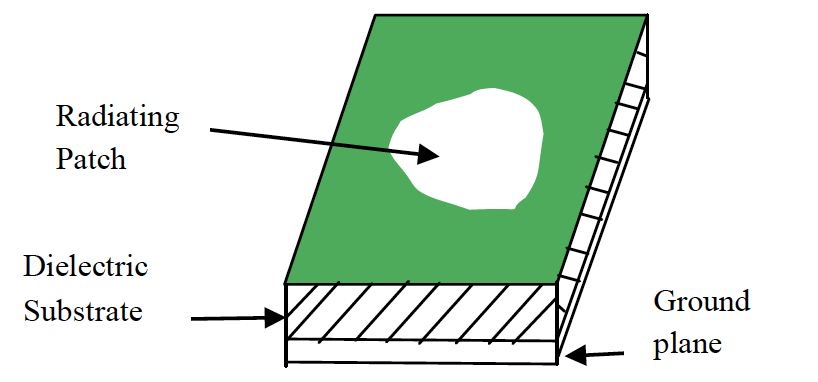
\includegraphics[width=\textwidth/2]{../images/patchantenna.png}
  \caption{General design of a microstrip antenna}
  \label{fig:basicpatchantenna}
\end{figure}

The microstrip antenna requires besides the groundplane, dielectric substrate and the radiation patch also a feed line. Several feeding techniques exist of which the most popular are: coaxial probe feeding, microstrip line and aperture coupling. %and Microstrip Patch Antenna
%(todo: more refs? gebruik nummer twee van J13 (p2))

A first feeding method is with the usage of a coaxial cable where the outer conductor is attached to the ground plane and the inner conductor to the radiations patch. Modelling is however difficult, especially for thick substrates as will be used in this master dissertation.
A second option is the usage of a microstrip line. This type of feeding is much easier to model since the microstrip line can be seen as en extension of the radiating patch.
A disadvantage is the increased \gls{spuriousradiation} which limits bandwith.
A third is proximity coupling which has the largest bandwidth and low \gls{spuriousradiation}. It consist however of two dielectric substrates causing the overall thickness
of the antenna to increase as well as it's fabrication difficulty.
%(todo: tekst te weinig, bespreek ook apperture coupled attenna (zelfde paper als de rest))

The increasing usage of the microstrip patch antennae can be explained by it's easy fabrication and lightweightness and therefore knows a widespread application in the millitary, global possitioning systems, telemedicine, WiMax applications and so on.
The authors of \cite{J13_microstripadvantages} also state that some of the disadvantages like lower gain and power handling can be solved with the usage of an array configuration.

The radiating patch is usually made of a thin layer of either gold or copper \cite{J14_antennadesign,J15_antennadesign}
and can be any form. However, shapes besides a circle or rectangle would require large numerical computation \cite{J14_antennadesign}.
A simple rectangular shape will thus be used.
Further is also the dielectric constant of the substrate important which typically varies between 2.2 and 12. Finding a good dielectric depends on how the antenna will used. A lower
dielectric constant with a thick substrate will result in better performance, better efficiency and larger bandwidths  \cite{J15_antennadesign}.
On the other hand, a larger dielectric constant reduce de dimensions of the antenna \cite{J14_antennadesign}
which is also useful when attaching the 
antenna to a limited surface. Glass as a dielectric substrate with a constant of 4.4 will be used.